\documentclass[letterpaper]{article}
\usepackage[margin=1in]{geometry}
\usepackage[utf8]{inputenc}
\usepackage{textcomp}
\usepackage{amssymb}
\usepackage{natbib}
\usepackage{graphicx}
\usepackage{gensymb}
\usepackage{amsthm, amsmath, mathtools}
\usepackage[dvipsnames]{xcolor}
\usepackage{enumerate}
\usepackage{mdframed}
\usepackage[most]{tcolorbox}
\usepackage{csquotes}
% https://tex.stackexchange.com/questions/13506/how-to-continue-the-framed-text-box-on-multiple-pages

\tcbuselibrary{theorems}

\newcommand{\R}{\mathbb{R}}
\newcommand{\Z}{\mathbb{Z}}
\newcommand{\N}{\mathbb{N}}
\newcommand{\Q}{\mathbb{Q}}
\newcommand{\C}{\mathbb{C}}
\newcommand{\code}[1]{\texttt{#1}}
\newcommand{\mdiamond}{$\diamondsuit$}
\newcommand{\PowerSet}{\mathcal{P}}
\newcommand{\Mod}[1]{\ (\mathrm{mod}\ #1)}
\DeclareMathOperator{\lcm}{lcm}

%\newtheorem*{theorem}{Theorem}
%\newtheorem*{definition}{Definition}
%\newtheorem*{corollary}{Corollary}
%\newtheorem*{lemma}{Lemma}
\newtheorem*{proposition}{Proposition}


\newtcbtheorem[number within=section]{theorem}{Theorem}
{colback=green!5,colframe=green!35!black,fonttitle=\bfseries}{th}

\newtcbtheorem[number within=section]{definition}{Definition}
{colback=blue!5,colframe=blue!35!black,fonttitle=\bfseries}{def}

\newtcbtheorem[number within=section]{corollary}{Corollary}
{colback=yellow!5,colframe=yellow!35!black,fonttitle=\bfseries}{cor}

\newtcbtheorem[number within=section]{lemma}{Lemma}
{colback=red!5,colframe=red!35!black,fonttitle=\bfseries}{lem}

\newtcbtheorem[number within=section]{example}{Example}
{colback=white!5,colframe=white!35!black,fonttitle=\bfseries}{def}

\newtcbtheorem[number within=section]{note}{Important Note}{
        enhanced,
        sharp corners,
        attach boxed title to top left={
            xshift=-1mm,
            yshift=-5mm,
            yshifttext=-1mm
        },
        top=1.5em,
        colback=white,
        colframe=black,
        fonttitle=\bfseries,
        boxed title style={
            sharp corners,
            size=small,
            colback=red!75!black,
            colframe=red!75!black,
        } 
    }{impnote}
\usepackage[utf8]{inputenc}
\usepackage[english]{babel}
\usepackage{fancyhdr}
\usepackage[hidelinks]{hyperref}

\pagestyle{fancy}
\fancyhf{}
\rhead{Math 170B}
\chead{Monday, April 17, 2023}
\lhead{Lecture 7}
\rfoot{\thepage}

\setlength{\parindent}{0pt}

\begin{document}

\section{Newton's Method (Section 3.2)}
Newton's Method is an efficient iterative method for solving nonlinear equations, assuming it works. Let $r$ be a root of some function, and let $x$ be an approximation to $r$. Then, our goal is to find an estimate of $r$, or $r = x_{m + 1} = x_m + h$, where $x_{m + 1}, x_m, h \in \R$. If $f''$ exists and is continuous, then by the Taylor series, we have 
\[0 = f(r) = f(x_{m + 1}) = f(x_m) + hf'(x_m) + \BigO(h^2).\]
Then, $h = \frac{f(x_m)}{f'(x_m)}$ will be part of an updating scheme. For a sufficiently small $h$ (i.e., $x$ is near $r$), then we can reasonably ignore the $\BigO(h^2)$ term. 

\subsection{Newton Iteration in 1-Dimension}
For $m = 0, 1, 2, \hdots$, we have 
\[x_{m + 1} = x_m - \frac{f(x_m)}{f'(x_m)}.\]
In other words, Newton's method begins with an estimate $x_0$ of $r$, and then defines inductively. If we let $x_{m + 1} = x$, then the linearization at $x_m$ is 
\[f(x_{m + 1}) = f(x) \approx f(x_m) + (x - x_m) f'(x_m) = \ell(x) = 0.\]
\begin{center}
    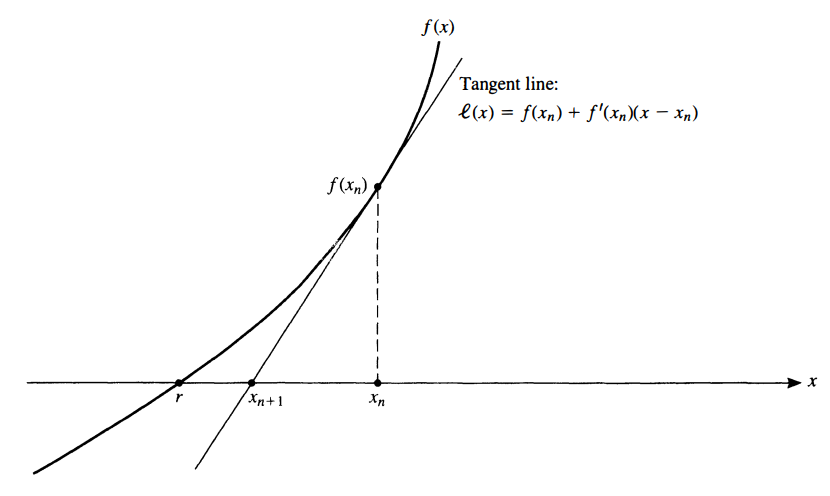
\includegraphics[scale=0.6]{../assets/geometric_newton.png}
\end{center}

\subsubsection{The Algorithm}
Let
\begin{itemize}
    \item $M$: the maximum number of iterations. 
    \item $\delta$: the step tolerance such that $|x_{m + 1} - x_m| < \delta$. 
    \item $\epsilon$: the convergence tolerance $|f(x_{m + 1})| < \epsilon$.
\end{itemize}
With a suitable $x_0$ being the starting point, the algorithm is as follows.

\begin{algorithm}[H]
    \caption{Newton's Algorithm}
    \label{alg:two}
    \begin{algorithmic}[1]
        \Function{Newton}{$x_0, M, \delta, \epsilon$}
            \State $v \gets f(x_0)$
            \If{$|v| < \epsilon$}
                \State \Return 
            \EndIf

            \For{$k \gets 1$ to $M$}
                \State $x_1 \gets x_0 - \frac{v}{f'(x_0)}$
                \State $v \gets f(x_1)$
                \If{$|x_1 - x_0| < \delta$ or $|f(x_1)| < \epsilon$}
                    \State \textbf{break}
                \EndIf

                \State $x_0 \gets x_1$
            \EndFor 
            \State \Return $v$
        \EndFunction
    \end{algorithmic}
\end{algorithm}
One thing to note: the algorithm will fail if $f'(x_0) = 0$ due to the division in line 7. 

\subsubsection{Requirements}
Defining the correct starting point $x_0$ is important. A bad starting point can result in nonconvergence.

\bigskip 

The function itself also matters. Other problems include when $f'(x_0) = 0$ or $f'(x_0)$ is infinite.

\begin{mdframed}
    (Example.) Consider the following function, 

    \begin{center}
        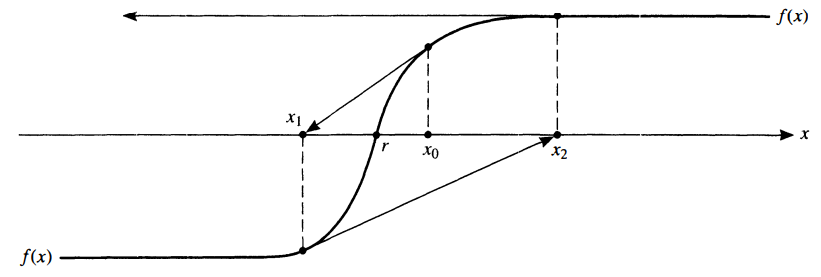
\includegraphics[scale=0.6]{../assets/newton_bad.png}
    \end{center}
    For this function, if $|x_0 - r| < |x_1 - r|$, then $|x_m - r| < |x_{m + 1} - r|$ and nonconvergence happens. In particular, the shape of the curve is such that for certain starting values, the sequence $[x_n]$ diverges.
\end{mdframed}

\subsubsection{Error Analysis}
Let the error be defined by $e_m = x_m - r$. Assume that $f(r) = 0 \neq f'(r)$ and $f''$ is continuous. Then, 
\[\begin{aligned}
    e_{m + 1} &= x_{m + 1} - r \\ 
        &= \left(x_m - \frac{f(x_m)}{f'(x_m)}\right) - r \\
        &= e_m - \frac{f(x_m)}{f'(x_m)} \\ 
        &= \frac{e_m f'(x_m) - f(x_m)}{f'(x_m)}.
\end{aligned}\]
We can now incorporate a Taylor expansion, 
\[0 = f(r) = f(x_m - e_m) = f(x_m) - e_m f'(x_m) + \frac{1}{2}e_m^2 f''(\xi)\]
for some aribitrary $\xi$ between $x_m$ and $r$ that makes the equation equal. Then, 
\begin{equation*}
    \begin{aligned}
        -(f(x_m) - e_m f'(x_m)) &= \frac{1}{2}e_m^2 f''(\xi) \\ 
            &\implies e_{m + 1} = \frac{\frac{1}{2} e_m^2 f''(\xi_m)}{f'(x_m)} \\ 
            &\implies e_{m + 1} \approx Ce_m^2,
    \end{aligned}
\end{equation*}
where $C$ is a bound of $\frac{\frac{1}{2} f''(\xi_m)}{f'(x_m)}$. So, in Newton's method, we have a quadratic convergence so that $e_{m + 1} \leq Ce_m^2$ or $|x_{m + 1} - r| \leq C |x_m - r|^2.$ 

\bigskip 

\textbf{Remark:} If $f$ is $C^2 (\R)$ is increasing, is convex (i.e., $f''(x) > 0$ for all $x$), and has a zero, then Newton's Method converges to it from any starting point.

\begin{mdframed}
    (Example.) Let $R > 0$ and $x = \sqrt{R}$. Then, 
    \[f(x) = x^2 - R = 0\] and \[f'(x) = 2x.\] Then, the iteration corresponds to \[x_{m + 1} = x_m - \frac{f(x_m)}{f'(x_m)} = x_m - \frac{x_m^2 - R}{2x_m} = \frac{1}{2}\left(x_m + \frac{R}{x_m}\right).\] 
\end{mdframed}

\subsection{Newton Iteration in 2-Dimensions}
Suppose $f_{1}(x_1^*, x_2^*) = 0$ and $f_{2}(x_1^*, x_2^*) = 0$. In other words, we have two variables and two functions. The goal is to linearize $x_1^* = x_i + h_i$, where $h_i$ is some small pertubation (error) and $1 \leq i \leq 2$. Then,
\[0 = f_{1}(x_1^*, x_2^*) = f_{1}(x_1 + h_1, x_2 + h_2) \approx f_{1}(x_1, x_2) + h_1 \frac{\partial f_1}{\partial x_1} + h_2 \frac{\partial f_1}{\partial x_2}\]

\[0 = f_{2}(x_1^*, x_2^*) = f_{2}(x_1 + h_1, x_2 + h_2) \approx f_{2}(x_1, x_2) + h_1 \frac{\partial f_2}{\partial x_1} + h_2 \frac{\partial f_2}{\partial x_2}.\]
From there, we can create a system 
\[\begin{bmatrix}
    0 \\ 0
\end{bmatrix} = \begin{bmatrix}
    f_{1}(x_1, x_2) \\ 
    f_{2}(x_1, x_2)
\end{bmatrix} + \underbrace{\begin{bmatrix}
    \frac{\partial f_1}{\partial x_1} & \frac{\partial f_1}{\partial x_2} \\ 
    \frac{\partial f_2}{\partial x_1} & \frac{\partial f_2}{\partial x_2}
\end{bmatrix}}_{J} \begin{bmatrix}
    h_1 \\ h_2
\end{bmatrix}.\]
Here, the $J$ is the Jacobian matrix. The goal is to solve for $\begin{bmatrix}
    h_1 \\ h_2
\end{bmatrix}$. By subtracting a term from the above equation, we have 
\[\begin{bmatrix}
    f_{1}(x_1, x_2) \\ 
    f_{2}(x_1, x_2)
\end{bmatrix} = -J\begin{bmatrix}
    h_1 \\ h_2
\end{bmatrix} \implies (-J)^{-1}\begin{bmatrix}
    f_{1}(x_1, x_2) \\ 
    f_{2}(x_1, x_2)
\end{bmatrix} = \begin{bmatrix}
    h_1 \\ h_2
\end{bmatrix}.\]
The iteration, then, is 
\[\begin{bmatrix}
    x_{1}^{(k + 1)} \\ 
    x_{2}^{(k + 1)}
\end{bmatrix} = \begin{bmatrix}
    x_{1}^{(k)} \\ 
    x_{2}^{(k)}
\end{bmatrix} + \begin{bmatrix}
    h_1^{(k)} \\ 
    h_2^{(k)}
\end{bmatrix} \qquad k \geq 0.\]
\textbf{Remarks:}
\begin{itemize}
    \item Just like in the one-dimensional case where $f'(x_0) \neq 0$, for this iterative formula to be well-defined, the Jacobian matrix must be nonsingular.
    \item The vector, $\begin{bmatrix}
        h_1 \\ h_2
    \end{bmatrix}$, is computed by solving a system (e.g., using Gaussian elimination).
\end{itemize}

\subsection{Generalization to Many Dimensions}
Given $m$ variables and $m$ equations, then 
\[f_{i}(x_1, x_2, \hdots, x_m) = 0 \qquad 1 \leq i \leq m.\]
Then, 
\[F = \begin{bmatrix}
    f_1 \\ f_2 \\ \vdots \\ f_m
\end{bmatrix}, \quad X = \begin{bmatrix}
    x_1 \\ x_2 \\ \vdots \\ x_m 
\end{bmatrix}, \quad H = \begin{bmatrix}
    h_1 \\ h_2 \\ \vdots \\ h_m
\end{bmatrix}.\]
Then, we can linearize the vector function, 
\[0 = F(X + H) \approx F(X) + F'(X)H,\]
where 
\[F'(x) = J(x) = \begin{bmatrix}
    \frac{\partial f_1}{\partial x_1} & \frac{\partial f_1}{\partial x_2} & \hdots & \frac{\partial f_1}{\partial x_m} \\ 
    \frac{\partial f_2}{\partial x_1} & \frac{\partial f_2}{\partial x_2} & \hdots & \frac{\partial f_2}{\partial x_m} \\ 
    \vdots & \vdots & \ddots & \vdots \\ 
    \frac{\partial f_m}{\partial x_1} & \frac{\partial f_m}{\partial x_2} & \hdots & \frac{\partial f_m}{\partial x_m}
\end{bmatrix} \in \R^{m \times m}.\]
So, Newton's method for $m$ nonlinear equations in $m$ variables is given by \[X^{(k + 1)} = X^{(k)} + H^{(k)},\]
where the Jacobian system is 
\[\underbrace{F'(X^{(k)})}_{J(X^{(k)})} H^{(k)} = -F(X^{(k)}).\]

\subsubsection{The Algorithm}
So, in the iterative algorithm, we have 
\[J(X^{(k)}) H^{(k)} = -F(X^{(k)}).\] 
Recall that $X^{(k + 1)} = X^{(k)} + H^{(k)}$. With this in mind, our algorithm takes in the following: 
\begin{itemize}
    \item $M$: the maximum number of iterations. 
    \item $\epsilon$: the tolerance, $||F(x^{(k)})||_2 \leq \epsilon$
    \item $\delta$: the step, $||x^{(k + 1)} - x^{(k)}||_2 \leq \delta$. 
\end{itemize}

\begin{algorithm}[H]
    \caption{Newton's Algorithm in Multiple Dimensions}
    \label{alg:three}
    \begin{algorithmic}[1]
        \Function{Newton}{$X^{(0)}, M, \epsilon, \delta$}
            \State $X^{(k)} \gets X^{(0)}$
            \State $F^{(k)} = F(X^{(k)})$
            \For{$k \gets 1$ to $M$}
                \State $J^{(k)} \gets F'(X^{(k)})$
                \State $H^{(k)} \gets -J^{(k)} \backslash F^{(k)}$ \Comment{Solve the system.}
                \State $X^{(k)} \gets X^{(k)} + H^{(k)}$
                \State $F^{(k)} \gets F(X^{(k)})$
                \If{$||F^{(k)}||_2 \leq \epsilon$ or $||H^{(k)}||_2 \leq \delta$}
                    \State \textbf{break} 
                \EndIf
            \EndFor 
            \State \Return $X^{(k)}$
        \EndFunction
    \end{algorithmic}
\end{algorithm}

\begin{mdframed}
    (Example.) Suppose we have \[F(x) = \begin{bmatrix}
        x_1 x_2 - x_3^2 - 1 \\ 
        x_1 x_2 x_3 - x_1^2 + x_2^2 - 2 \\ 
        e^{x_1} - e^{x_2} + x_3 - 3
    \end{bmatrix} = 0\]
    and $X^{(0)} = \begin{bmatrix}
        1\\1\\1
    \end{bmatrix}.$ Then, 
    \[F'(x) = J(x) = \begin{bmatrix}
        x_2 & x_1 & -2x_3 \\ 
        x_2 x_3 - 2x_1 & x_1 x_3 + 2x_2 & x_1 x_2 \\
        e^{x_1} & -e^{x_2} & 1
    \end{bmatrix}.\]
\end{mdframed}


\end{document}